\chapter{System Implementation} \label{s-i}

\section{Introduction} \label{s-i--introduction}

This chapter describes how the system was implemented based on the previous artefact design. From design to implementation a few decisions and technologies changed.

Figure \ref{figure-application-stack-implementation}, shows the revised application stack for the implementation.

\begin{figure}[H]
  \centering
    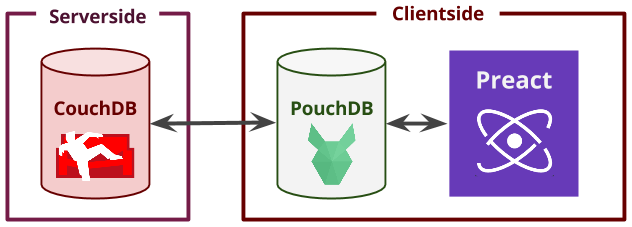
\includegraphics[width=\textwidth,height=\textheight,keepaspectratio]{application_stack_implementation}
  \caption{Overview of how the application stack is structured for the implementation}
  \label{figure-application-stack-implementation}
\end{figure}

The biggest change was the removal of Node.js stack including Express and Passport. As explained fully in section \ref{s-i--data-and-databases} the data manipulation and authentication functionality were handled through CouchDB.

\section{Packages} \label{s-i--packages}

During implementation and research into React and performance another framework was discovered called Preact. Preact, is a framework that attempts to recreate functionality of React but with the focus of performance. Using Preact means a better development experience. \cite{preact} Preact is 3kb in size in comparison to React which is 53kb in size.

The implementation therefore used Preact and was used for rendering views in the artefact.

One principle for software development is DRY (don't repeat yourself). One principle for software development is DRY (don't repeat yourself). ``Every piece of knowledge must have a single, unambiguous, authoritative representation within a system.'' \cite{DRY}

A good example of this is the `moment.js' package used in this artefact, this package handles most date and time related problems. To implement these features is not inherently difficult, but packages such as moment.js offer DRY tried and tested solutions. \cite{moment.js}

\section{Service Worker and Offline Functionality} \label{s-i--sw-offline}

Offline caching of files was implemented through service worker. At the time of writing, there is discussion as to whether service worker is too low level for using the caching functionality. It is argued that this functionality could be brought through as a separate caching API. \cite{sw_sledgehammer}

Implementing the caching with service worker wasn't trivial but once learnt was understandable. Having a abstracted caching API could be useful for simpler implementations of offline caching.

Having a clientside database through PouchDB and IndexedDB (as further discussed in section \ref{s-i--data-and-databases}) not only does this mean offline data but also quick retrieval of data even when connected to a network. This is a boost for performance in general.

\section{Data and Databases} \label{s-i--data-and-databases}

As previously mentioned CouchDB is excellent at master-to-master replication of databases. This means syncing is easily implemented.

The remote database and the local databases sync any changes between themselves, when the local database changes the recipes and brews in state are updated.

In the artefact design data section \ref{a-d--data} and following the decision was to use Node for a Express to handle data coming from the database and Passport to handle user authentication. However through the use of CouchDB and PouchDB it was found that there was no need for either of these technologies.

CouchDB has a user authentication system for handling permission and roles to documents. By default everyone is an admin in what they describe as the `admin party', this is recommended to be disabled but aids development with low barrier to entry when starting a new project.

As the data defines a lot of the structure of the application this authentication system has been leveraged for user authentication for the application.

\section{Interesting Problems} \label{s-i--interesting-problems}

\begin{figure}[H]
  \centering
    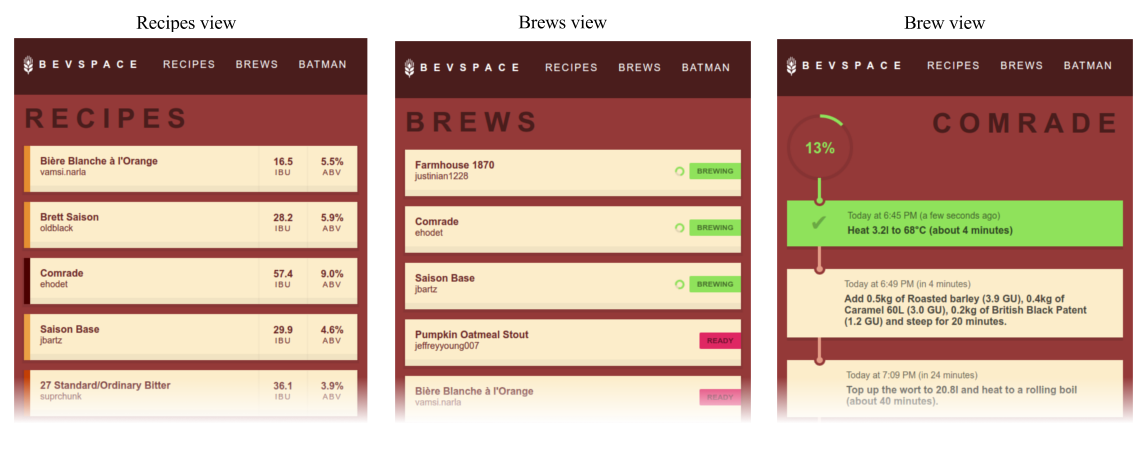
\includegraphics[width=\textwidth,height=\textheight,keepaspectratio]{implementation}
  \caption{Screenshots of different views as implemented}
  \label{figure-implementation-screenshots}
\end{figure}

During the implementation of this project several issues came up. This section discusses some of these issues.

Using newer technologies such as Webpack, ESLint, Babel and Preact come with difficulties. There is a generally a lack of support found online and even some issues can be so new they haven't been documented yet.

For example, with Preact during implementation there was an issue with a feature from React not being supported. This was short-circuit boolean templating, the author then reported this bug which was then fixed. Here having the Preact project as an Open Source project meant this could be fixed not just for this artefact but future users of Preact.

While testing the service worker code and implementation difficulties arise when caching files. Originally the author was manually unregistering the service worker then closing and reopening the tab.

Simply refreshing does not give you any updated version of the service worker files, this is due to the browser making the new page request before unloading the current page so the activated service worker is never released. \cite{refresh_sw}

As shown in Figure \ref{figure-force-update-service-worker}, to solve this problem there is a `Force update on page load' option in the Chrome development tools.

\begin{figure}[H]
  \centering
    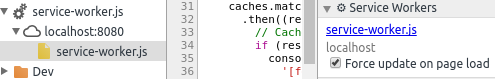
\includegraphics[width=\textwidth,height=\textheight,keepaspectratio]{force_update_service_worker}
  \caption{The `force update on page load' option}
  \label{figure-force-update-service-worker}
\end{figure}

One issue with frameworks and libraries expressed in section \ref{l-r--frameworks} was the lack of control of final code. Having to depend on the Brauhaus package due to a lack of home-brewing knowledge resulted in having to implement more of the library than potentially needed and ultimately a bigger file size reducing performance.

Keeping dependencies up to date is important mostly for security (see Snyk mentioned in section \ref{t-e--testing}), a tool called Greenkeeper (shown in Figure \ref{figure-greenkeeper}) was used through-out which monitors the project's dependencies and sends a Pull Request to the GitHub repository with an updated version of packages. This is great as these Pull Requests can be run through the continuous integration and if it passes the build can be merged straight away. \cite{greenkeeper}

\begin{figure}[H]
  \centering
    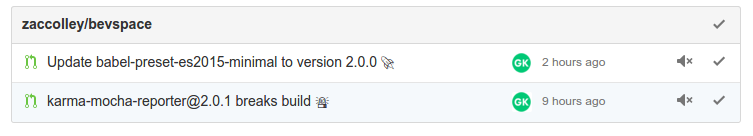
\includegraphics[width=\textwidth,height=\textheight,keepaspectratio]{greenkeeper}
  \caption{Example of Greenkeeper testing different package updates}
  \label{figure-greenkeeper}
\end{figure}

One problem when developing with service workers (and other web APIs) is needed SSL or https when in production. Thankfully, \verb|localhost| is ignored so these features can be used in development easily. Also with projects such as Let's Encrypt, adding SSL to a web site is free and easy. \cite{letsencrypt}

\section{Summary} \label{s-i--summary}

This chapter described the change in technology stack, interesting problems surrounding working with newer technologies such as service worker. It also discusses tools and packages used for the implementation and their benefits.
